\subsection{Matrix-Verteilung}

Um die Matrix vom Root-Prozess an die anderen Prozesse im Cluster zu verteilen, werden im wesentlichen 2 MPI-Aufrufe genutzt. Die Implementierung ist in der folgenden Datei zu finden:

\begin{lstlisting}[language=C, aboveskip=\baselineskip, basicstyle=\footnotesize\ttfamily, lineskip=0pt]
find_components.c:
	static int mpi_distribute_matrix(struct processor_data *pdata, int *dims, matrix_type *input_matrix)
	static int mpi_working_function(struct processor_data *pdata, int *dims)
\end{lstlisting}

Zuerst werden mittels \verb+MPI_Scatterv+ die Dimensionen der zu übertragenen Matrizen verteilt, die anderen Prozesse im Cluster allozieren daraufhin genügend Speicher für die Matrizen. Danach werden mittels speziell angelegter MPI-Datentypen die einzelnen Matrix-Teile übermittelt (verwendet wird \verb+MPI_Type_vector+, um eine Teilmatrix-Zeile zu adressieren). Durch die verwendeten MPI-Datentypen ist es möglich, dass jeder Matrix-Teil nur eine Sende-Operation benötigt.

Leider ist es bei den verwendeten Datenstrukturen nicht möglich Gruppen-Operationen zu verwenden, um die Matrix-Teile zu senden. Die einzige Operation die in Frage kommen würde, ist \verb+MPI_Scatterv+, aber \verb+scatterv+ verwendet ein unzureichendes Displacement (eine nähere Erläuterung dazu ist an der entsprechenden Stelle im Quell-Code hinterlegt).

\subsection{Komponenten-Ermittlung} \label{algorithm:find_components}

Der wesentliche Teil des Programms ist die Ermittlung der vorhandenen Komponenten in einer (Teil-)Matrix. Die Implementierung des Algorithmus befindet sich im wesentlichen in:

\begin{lstlisting}[language=C, aboveskip=\baselineskip, basicstyle=\footnotesize\ttfamily, lineskip=0pt]
components.c, components.h:
	int find_components(matrix_type *mat, struct component_list **comp_list, vector_type **borders)

helper/{matrixgraph.c, matrixgraph.h}
\end{lstlisting}

\verb+find_components()+ fasst das gegebe Problem der Komponenten-Ermittlung als Graphen-Problem auf. Dazu wird die Matrix in einen Graphen überführt (siehe Abbildung \ref{fig:matrix_graph} auf Seite \pageref{fig:matrix_graph}).

\begin{figure}[tbhp]
	\centering
	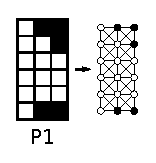
\includegraphics[width=0.4\textwidth]{images/matrix_graph.eps}
	\caption{Beispiel für die Umwandlung einer Matrix in einen Graphen}
	\label{fig:matrix_graph}
\end{figure}

Im überführten Graphen befinden sich dann Knoten mit dem Wert 0 und 1 - für weiß und schwarz. Auf diesen Graphen wird wie folgt eine Tiefensuche angewendet:

Jeder Knoten erhält eine Farbe (nicht zu verwechseln mit der Farbe der Komponenten; zu Anfang ist jeder Knoten weiß). Danach wird zunächst ein Knoten auf einen Stack gepusht. Mit dieser Push-Operation wird der Knoten außerdem grau gefärbt. Dadurch kann erkannt werden, ob ein Knoten schon auf dem Stack liegt (ohne den Stack zu durchsuchen). Danach läuft der Algorithmus so lange, bis der Stack keine Knoten mehr enthält.

Jede Runde wird ein Knoten vom Stack geholt und expandiert - alle verbundenen Knoten, die noch weiß sind, werden auf den Stack gepusht und es wird untersucht, ob die Knoten den Wert 1 enthalten (also schwarze Pixel in der Matrix sind). Sollte ein Knoten mit Wert 1 vorhanden sein, der noch keiner Komponente zugeordnet ist (die Knoten enthalten neben dem Wert auch die Komponenten-ID), wird eine neue Komponente angelegt und dem Knoten zugeordnet. Außerdem wird eine weitere Tiefen-Suche gestartet, die das Ziel hat, die neue Komponente zu vervollständigen (\verb+complete_component()+). Als letztes wird der Knoten, der vom Stack geholt wurde, schwarz gefärbt und aus dem Graphen entfernt, somit wird er nie wieder betrachtet. Ein Beispiel für eine solche Expandierung ist in Abbildung \ref{fig:node_expand} auf Seite \pageref{fig:node_expand} zu sehen.

\begin{figure}[tbhp]
	\centering
	\includegraphics[width=0.5\textwidth]{images/node_expand.eps}
	\caption{Beispiel für das Expandieren eines Knotens}
	\label{fig:node_expand}
\end{figure}

Wenn keine Knoten mehr auf dem Stack sind, ist der Graph komplett durchsucht und alle Komponenten sind gefunden. Da jeder Knoten nur einmal expandiert wird und jeder Knoten eine feste Anzahl von verbundenen Knoten hat (gegeben durch die Entstehung des Graphen), ist die Laufzeit im schlechtesten Fall linear: $O(n*m)$ (in den Messungen, die im Abschnitt \ref{bench:task} auf Seite \pageref{bench:task} vorgestellt werden, kann auch das beobachtet werden).

\subsection{Randabgleich}

Der Abgleich der Rändern zweier aneinanderliegender Matrix-Teile ist in zwei Teile aufgeteilt. Die Implementierung ist aufgeteilt in:

\begin{lstlisting}[language=C, aboveskip=\baselineskip, basicstyle=\footnotesize\ttfamily, lineskip=0pt]
/* Kommunikation */
find_components.c:
	static int mpi_working_function(struct processor_data *pdata, int *dims);

/* Algorithmus zum Abgleich der Raender */
border_compare.c border_compare.h:
	int find_common_components(struct component_list *own_compl, struct component_list *communication_compl, matrix_type *compare_border, matrix_type *send_border, matrix_type *alien_border);
\end{lstlisting}

Zuerst versucht jeder Prozessor von seinem Vorgänger die Daten über dessen lokale Matrix zu erhalten (wie oben schon beschrieben). Im Fall des ersten Prozessors erkennt der Prozessor mittels der angelegten MPI-Topologie und deren Koordinaten, dass er keinen Vorgänger hat und überspringt diese Phase.

\subsubsection{Kommunikation}

Zum Empfangen der Komponenten wird zuerst mittels \verb+MPI_Probe+ und \verb+MPI_get_count+ getestet, wie viele Komponenten übertragen werden sollen (somit reicht eine Sende-Operation, anstelle von zwei, um zuerst die Größe zu übertragen). Beim anschließenden blockierenden \verb+MPI_Recv+ wird ein eigener Typ verwendet, der für die übertragene Struktur angelegt wurde (\verb+MPI_component_type+, angelegt in \verb+register_mpi_component_type()+). Da die Komponenten von Anfang an in einem Vector gespeichert werden (siehe \ref{algorithm:ds} auf Seite \pageref{algorithm:ds}) und deshalb hintereinander im Speicher stehen, reicht eine Sende-Operation und eine einmalige Allozierung auf der Empfänger-Seite aus, um den Austausch der Komponenten abzuschließen.

Der Vorgänger überträgt danach noch den Rand, der an dem des aktuellen Knoten anliegt, damit der aktuelle Knoten zusammenhängende Komponenten erkennen kann (der Rand ist auch eine Matrix, mit nur einer Dimension, und enthält in seinen Feldern die ID der dort erkannten Komponente, siehe Abbildung \ref{fig:find_result} auf Seite \ref{fig:find_result}). Für diese Übertragung wird auch ein eigener MPI-Datentyp angelegt (\verb+border_type+) und es wird eine blockierende Sende-Operation verwendet (\verb$Send + Recv$).

\subsubsection{Abgleich}

Damit die Komponenten erkannt werden, die durch die Teilung der Matrix separiert wurden, wird vom jeweiligen Empfänger die Funktion \verb+find_common_components()+ benutzt. Diese Funktion vergleicht den empfangenen Rand des Vorgängers (ab hier: \textit{links}) mit dem Rand der eigenen Matrix (ab hier: \textit{rechts}), der an diesem anliegt. Dabei geht der Algorithmus den linken Rand von oben nach unten durch und vergleicht das aktuelle Feld mit den drei angrenzenden Feldern im rechten Rand.

Bei diesem Vergleich können folgende Fälle auftreten (jeweils, wenn links und rechts eine Komponente gefunden wird):
\begin{itemize}
	\item Die linke Komponente ist bisher noch nicht verbunden worden: die linke Komponente wird zur rechten hinzu addiert und entfernt. Diese Verbindung wird gespeichert.
	\item Die linke Komponente wurde schon einmal verbunden:
		\begin{itemize}
			\item Es liegt bereits eine Verbindung mit der rechten Komponente vor: keine weitere Aktion.
			\item Es liegt noch keine Verbindung mit der rechten Komponente vor: zwei der eigenen Komponenten werden durch die Fremde verbunden. Diese beiden müssen also verbunden werden und eine muss aus der eigenen Liste entfernt werden. Dabei muss beachtet werden, dass die entfernte Komponenten eventuell in dem Rand auftaucht, der an den Nachfolger des Knotens übertragen werden muss.
		\end{itemize}
\end{itemize}

Sobald der Algorithmus fertig ist, sind alle passenden Komponenten verbunden und der Rest der empfangenen Komponenten wird in die eigene Liste übernommen. Die eigene Liste wird danach an den nächsten Knoten versendet. Für den Fall, dass der aktuelle Knoten bereits der letzte ist, steht nun das Ergebnis zur Verfügung.

\subsection{Datenstrukturen} \label{algorithm:ds}

In allen Teilen des Programms wurden einige höhere Datenstrukturen verwendet, die es zum einen erleichtern sollen, den allozierten Speicher des Programms zu verwalten und zum anderen, den Zugriff auf den Speicher zu vereinheitlichen. Da C selbst keine solchen Datenstrukturen in seiner Standard-Bibliothek zur Verfügung stellt, wurden eigene entwickelt. Die Header-Dateien sind in:

\begin{lstlisting}[language=C, aboveskip=\baselineskip, basicstyle=\footnotesize\ttfamily, lineskip=0pt]
helper/vector.h
helper/list.h
helper/matrix.h
helper/stack.h
helper/queue.h
helper/matrixgraph.h /* spezieller Graph fuer dieses Programm */
helper/constvector.h /* spezielle Variante eines vectors, fuer eigene Allokatoren gedacht */
\end{lstlisting}

Verwendet wurden in dem Programm hauptsächlich:

\begin{itemize}
	\item \textsl{\textbf{Vector:}} 'dynamisches' Array. Auf \verb+vector->values+ wird Speicher alloziert (je nach Größe der zu speichernden Elemente), falls durch eine \verb+add+-Operation dieser Speicher überlaufen würde, wird er automatisch erweitert (\verb+realloc+).
	\item \textsl{\textbf{Matrix:}} ein verwaltetes zweidimensionales Array. Auf \verb+matrix->matrix+ wird genügend Speicher für $m \times n$ Elemente der angegebenen Größe alloziert, anschließend kann dieser Speicher nicht geschrumpft/vergrößert werden. Bei Zugriffen werden die Indizes überprüft, um Segmentation-Faults zu vermeiden.
	\item \textsl{\textbf{Stack:}} ein klassischer Stack, basierend auf einem Vector.
	\item \textsl{\textbf{Matrixgraph:}} eine spezielle Graphen-Struktur, die auf eine Matrix aufbaut. Dabei wird die Regelmäßigkeit einer Matrix ausgenutzt, so können Zugriffszeiten linear bleiben.
\end{itemize}

Bei all diesem Datenstrukturen ist zu beachten: Da C keine Form von Polymorphie unterstützt, müssen die Elemente der Strukturen als void-Pointer behandelt werden, da sonst keine allgemeinen Strukturen möglich sind. Das hat aber zur Folge, dass bei \verb+Get/Add/..+ Operationen keine Typ-Prüfung stattfinden kann. Diese Aufgabe muss der Programmierer übernehmen. In den Quelltexten dieses Programms wurde soweit möglich jede verwendete Datenstruktur mit dem gespeicherten Typ kommentiert.